\documentclass[border=10pt]{standalone}

\usepackage{tikz}
\usepackage{tikzsymbols}
\usetikzlibrary{calc,patterns,shapes.geometric}

\def\centerarc[#1](#2)(#3:#4:#5){\draw[#1] ($(#2)+({#5*cos(#3)},{#5*sin(#3)})$) arc (#3:#4:#5);}

\begin{document}
	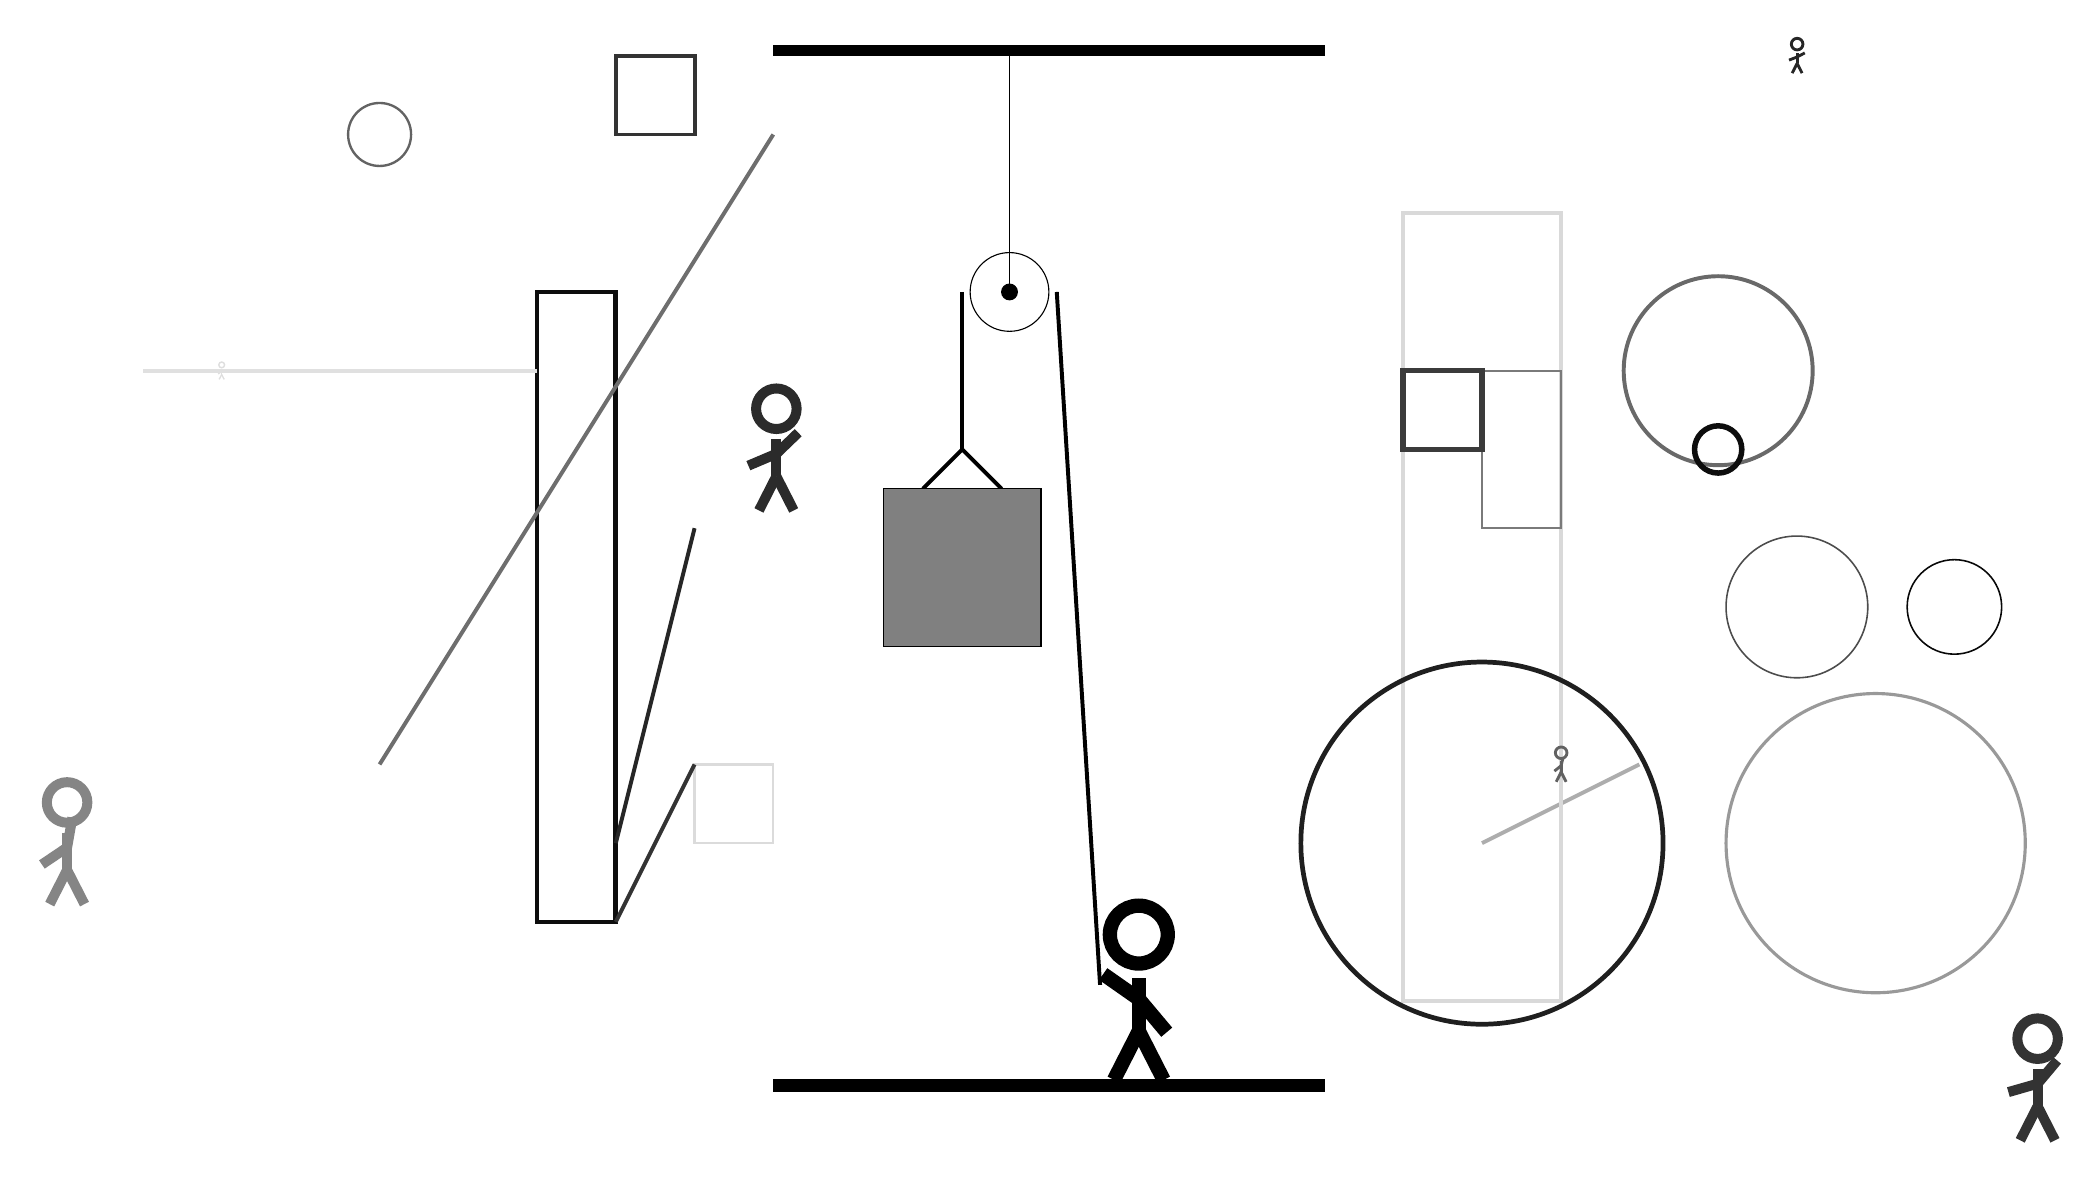
\begin{tikzpicture}
		%%%%% START %%%%%
		
		\draw[fill=black] (-2, 10) rectangle (5, 10.125);
		
		\draw (1, 7) circle (0.5);
		\draw[fill=black] (1, 7) circle (0.1);
		\draw (1, 10) -- (1, 7);
		
		\draw[line width=0.5mm] (-0.1, 4.5) -- (0.4, 5.0) -- (0.9, 4.5);
		\draw[fill=black!50] (-0.6, 4.5) rectangle (1.4, 2.5);
		
		\draw[line width=0.5mm] (0.4, 7) -- (0.4, 5.0);
		\centerarc[line width=0.5mm](1, 7)(0:180:0.6);
		\draw[line width=0.5mm](1.6, 7) -- (2.15, -1.8);
		
		\draw[line width=0.6mm, color=black!95] (-4, -1) rectangle (-5, 7);
		
		\draw[line width=0.5mm, color=black!85](-3, 4) -- (-4, 0);
		\node[line width=0.2mm, color=black!83] at (-2, 5) {\Strichmaxerl[7][23][44]};
		\draw[line width=0.5mm, color=black!80] (-3, 9) rectangle (-4, 10);
		\node[line width=0.2mm, color=black!13] at (-9, 6) {\Strichmaxerl[1][37][4]};
		\draw [line width=0.4mm, color=black!40](12, 0) circle (1.9);
		\draw [line width=0.3mm, color=black!61](-7, 9) circle (0.4);
		\draw [line width=0.2mm, color=black!97](13, 3) circle (0.6);
		\draw[line width=0.5mm, color=black!32](7, 0) -- (9, 1);
		
		\draw[line width=0.3mm, color=black!14] (-2, 1) rectangle (-3, 0);
		\draw[line width=0.5mm, color=black!15] (6, 8) rectangle (8, -2);
		\node[line width=0.4mm, color=black!48] at (-11, 0) {\Strichmaxerl[7][34][80]};
		\node[line width=0.7mm, color=black!80] at (14, -3) {\Strichmaxerl[7][16][50]};
		
		\draw[line width=0.3mm, color=black!52] (7, 4) rectangle (8, 6);
		\node[line width=0.4mm, color=black!85] at (11, 10) {\Strichmaxerl[2][21][28]};
		\node[line width=0.2mm, color=black!62] at (8, 1) {\Strichmaxerl[2][39][77]};
		
		\draw [line width=0.5mm, color=black!59](10, 6) circle (1.2);
		
		\draw [line width=0.7mm, color=black!95](10, 5) circle (0.3);
		\draw[line width=0.7mm, color=black!77] (6, 5) rectangle (7, 6);
		\draw [line width=0.2mm, color=black!70](11, 3) circle (0.9);
		\draw [line width=0.3mm, color=black!23](10, 5) circle (0.0);
		
		\draw [line width=0.6mm, color=black!88](7, 0) circle (2.3);
		\draw[line width=0.5mm, color=black!80](-4, -1) -- (-3, 1);
		\draw[line width=0.5mm, color=black!12](-5, 6) -- (-10, 6);
		\draw[line width=0.5mm, color=black!57](-7, 1) -- (-2, 9);
		
		
		\node at (2.6, -1.9) {\Strichmaxerl[10][-35][-50]};
		
		\draw[fill=black] (-2, -3) rectangle (5, -3.15);
		
		%%%%% END %%%%%
	\end{tikzpicture}
\end{document}